\documentclass[10pt,a4paper,twoside]{report}
\usepackage[utf8]{inputenc}
%Algemene documentinstellingen als dubbelzijdig, codering, rapportsoort etc.

\usepackage{import} %Om het rapport in verschillende delen op te delen en in één bestand te importeren
\usepackage{preamble} %Importeert alle instellingen in preamble.sty


\begin{document}

\includepdf{./Titelpagina/omslag.pdf} %Omslagblad

\includepdf{./Titelpagina/legepagina.pdf} %Lege pagina na omslag
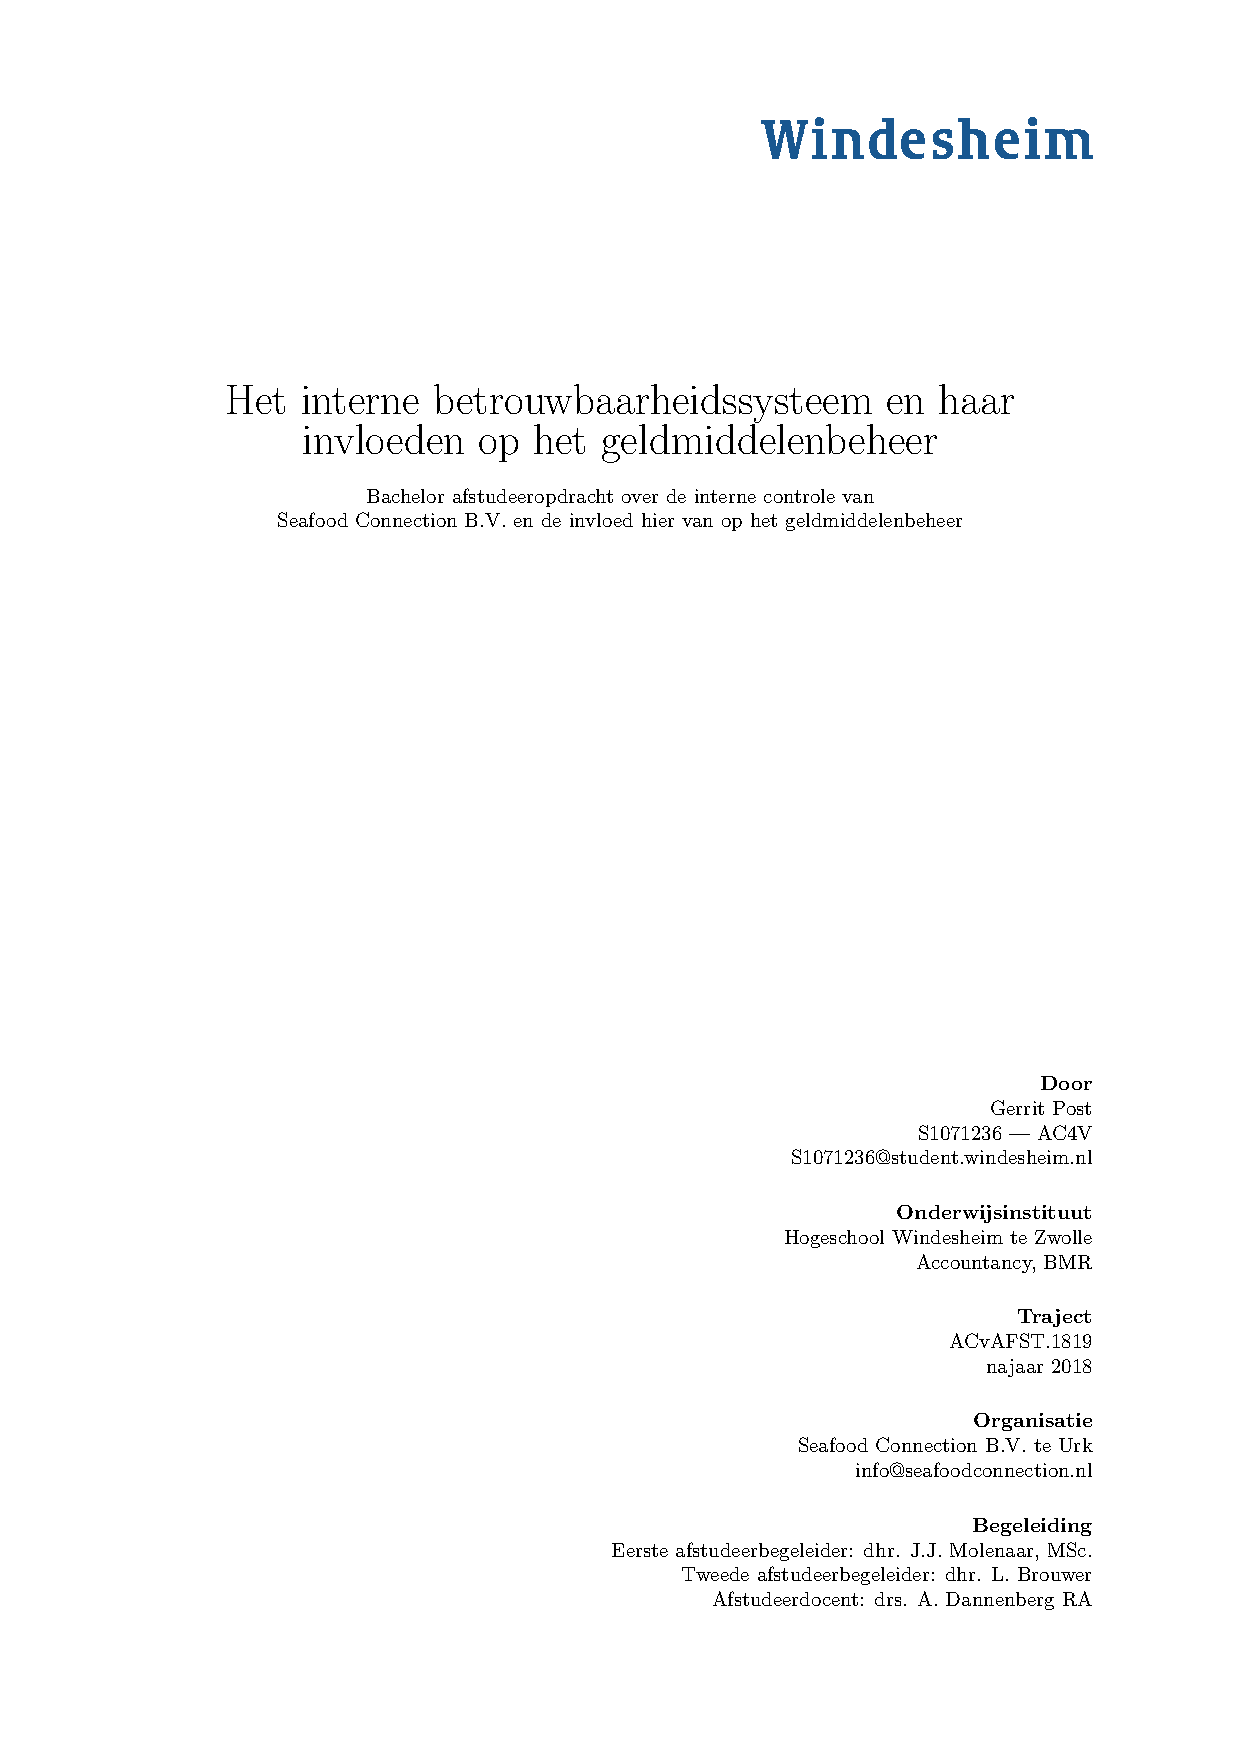
\includepdf{./Titelpagina/titelpagina.pdf} %Titelpagina
%De eerste drie pagina's worden geïmporteerd als PDF want deze pagina's zijn oneside in de preamble en dit Tex-bestand is twoside, zie eerste regel

\import{./Hoofdstukken/}{A-Voorwoord.tex}
\import{./Hoofdstukken/}{B-Samenvatting.tex}

\setcounter{page}{5} %Door importeren van PDF klopt paginanummer niet, hierbij gecorrigeerd
\tableofcontents
\thispagestyle{empty} %Geen paginanummer op de pagina van de ToC

\import{./Hoofdstukken/}{C-Inleiding.tex}
\import{./Hoofdstukken/}{Dk-Bedrijfsachtergrond.tex}
\import{./Hoofdstukken/}{E-Probleemanalyse.tex}
\import{./Hoofdstukken/}{F-Methode.tex}
\import{./Hoofdstukken/}{G-Resultaten.tex}
\import{./Hoofdstukken/}{H-Conclusie.tex}

%\listoffigures
%\listoftables
\printbibliography
\addcontentsline{toc}{chapter}{Bibliografie} %Ongenummerde hoofdstukken komen niet in ToC, met deze code wel

\import{./Hoofdstukken/}{Z-Bijlagen.tex}
\end{document}